%Version 3.1 December 2024
% See section 11 of the User Manual for version history
%
%%%%%%%%%%%%%%%%%%%%%%%%%%%%%%%%%%%%%%%%%%%%%%%%%%%%%%%%%%%%%%%%%%%%%%
%%                                                                 %%
%% Please do not use \input{...} to include other tex files.       %%
%% Submit your LaTeX manuscript as one .tex document.              %%
%%                                                                 %%
%% All additional figures and files should be attached             %%
%% separately and not embedded in the \TeX\ document itself.       %%
%%                                                                 %%
%%%%%%%%%%%%%%%%%%%%%%%%%%%%%%%%%%%%%%%%%%%%%%%%%%%%%%%%%%%%%%%%%%%%%

%%\documentclass[referee,sn-basic]{sn-jnl}% referee option is meant for double line spacing

%%=======================================================%%
%% to print line numbers in the margin use lineno option %%
%%=======================================================%%

%%\documentclass[lineno,pdflatex,sn-basic]{sn-jnl}% Basic Springer Nature Reference Style/Chemistry Reference Style

%%=========================================================================================%%
%% the documentclass is set to pdflatex as default. You can delete it if not appropriate.  %%
%%=========================================================================================%%

%%\documentclass[sn-basic]{sn-jnl}% Basic Springer Nature Reference Style/Chemistry Reference Style

%%Note: the following reference styles support Namedate and Numbered referencing. By default the style follows the most common style. To switch between the options you can add or remove “Numbered” in the optional parenthesis. 
%%The option is available for: sn-basic.bst, sn-chicago.bst%  
 
%%\documentclass[pdflatex,sn-nature]{sn-jnl}% Style for submissions to Nature Portfolio journals
%%\documentclass[pdflatex,sn-basic]{sn-jnl}% Basic Springer Nature Reference Style/Chemistry Reference Style
\documentclass[pdflatex,sn-mathphys-num]{sn-jnl}% Math and Physical Sciences Numbered Reference Style
%%\documentclass[pdflatex,sn-mathphys-ay]{sn-jnl}% Math and Physical Sciences Author Year Reference Style
%%\documentclass[pdflatex,sn-aps]{sn-jnl}% American Physical Society (APS) Reference Style
%%\documentclass[pdflatex,sn-vancouver-num]{sn-jnl}% Vancouver Numbered Reference Style
%%\documentclass[pdflatex,sn-vancouver-ay]{sn-jnl}% Vancouver Author Year Reference Style
%%\documentclass[pdflatex,sn-apa]{sn-jnl}% APA Reference Style
%%\documentclass[pdflatex,sn-chicago]{sn-jnl}% Chicago-based Humanities Reference Style

%%%% Standard Packages
%%<additional latex packages if required can be included here>

\usepackage{graphicx}%
\usepackage{multirow}%
\usepackage{amsmath,amssymb,amsfonts}%
\usepackage{amsthm}%
\usepackage{mathrsfs}%
\usepackage[title]{appendix}%
\usepackage{xcolor}%
\usepackage{textcomp}%
\usepackage{manyfoot}%
\usepackage{booktabs}%
\usepackage{algorithm}%
\usepackage{algorithmicx}%
\usepackage{algpseudocode}%
\usepackage{listings}%
\usepackage{fontspec}% XeTeX (tectonic): Unicode Computer Modern covers Cyrillic
\setmainfont{cmunrm.otf}[BoldFont=cmunbx.otf,ItalicFont=cmunti.otf,BoldItalicFont=cmunbi.otf]%
\setsansfont{cmunss.otf}[BoldFont=cmunsx.otf,ItalicFont=cmunsi.otf]\setmonofont{cmuntt.otf}%
\usepackage[ukrainian,english]{babel}%
\usepackage{url}%
%%%%

%%%%%=============================================================================%%%%
%%%%  Remarks: This template is provided to aid authors with the preparation
%%%%  of original research articles intended for submission to journals published 
%%%%  by Springer Nature. The guidance has been prepared in partnership with 
%%%%  production teams to conform to Springer Nature technical requirements. 
%%%%  Editorial and presentation requirements differ among journal portfolios and 
%%%%  research disciplines. You may find sections in this template are irrelevant 
%%%%  to your work and are empowered to omit any such section if allowed by the 
%%%%  journal you intend to submit to. The submission guidelines and policies 
%%%%  of the journal take precedence. A detailed User Manual is available in the 
%%%%  template package for technical guidance.
%%%%%=============================================================================%%%%

%% as per the requirement new theorem styles can be included as shown below
\theoremstyle{thmstyleone}%
\newtheorem{theorem}{Theorem}%  meant for continuous numbers
%%\newtheorem{theorem}{Theorem}[section]% meant for sectionwise numbers
%% optional argument [theorem] produces theorem numbering sequence instead of independent numbers for Proposition
\newtheorem{proposition}[theorem]{Proposition}% 
%%\newtheorem{proposition}{Proposition}% to get separate numbers for theorem and proposition etc.

\theoremstyle{thmstyletwo}%
\newtheorem{example}{Example}%
\newtheorem{remark}{Remark}%

\theoremstyle{thmstylethree}%
\newtheorem{definition}{Definition}%

\raggedbottom
%%\unnumbered% uncomment this for unnumbered level heads

%% reported numbers, generated from results/summary.json by scripts/08_build_paper.py
\newcommand{\NAudit}{??}
\newcommand{\NFableImages}{0}
\newcommand{\NGTNotVisible}{1\,719}
\newcommand{\NGTTokens}{11\,424}
\newcommand{\NImages}{567}
\newcommand{\NImgPerCell}{7}

\begin{document}
\title[Detecting text-reading hallucinations for blind users]{Detecting Text-Reading Hallucinations in Vision-Language Descriptions of Cyrillic Signage, Packaging and Documents for Blind Users}

\author*[1]{\fnm{Rostyslav} \sur{Zatserkovnyi}}\email{zatserkovnyi.rostyslav@gmail.com}

\author[2]{\fnm{Roksoliana} \sur{Zatserkovna}}\email{roksoliana.s.zatserkovna@lpnu.ua}

\affil*[1]{\orgname{Lviv University of Trade and Economics}, \orgaddress{\street{10 Tuhan-Baranovskyi Str.}, \city{Lviv}, \postcode{79008}, \country{Ukraine}}}

\affil[2]{\orgname{Lviv Polytechnic National University}, \orgaddress{\street{12 Stepan Bandera Str.}, \city{Lviv}, \postcode{79013}, \country{Ukraine}}}

\abstract{ABSTRACT-PLACEHOLDER}

\keywords{KW-PLACEHOLDER}

\maketitle


\section{Introduction}\label{sec:intro}

Reading text is one of the most frequent reasons blind people photograph their surroundings. The first crowd-powered visual question answering service, VizWiz, already found that a large share of questions asked what a label, sign or screen said~\cite{bigham2010vizwiz}, and later analyses of tens of thousands of such questions confirmed that reading and product identification dominate everyday visual needs~\cite{brady2013visual,gurari2018vizwiz}. Dedicated text readers such as Seeing AI and OrCam serve this need~\cite{granquist2021evaluation,khan2020insight}. Since 2023, general-purpose vision-language models (VLMs) have increasingly taken over the task. Scene-description apps built on these models let a blind user point a phone at a medicine box or a utility bill and receive a fluent spoken description~\cite{gonzalezpenuela2024investigating,xie2025beyond,adnin2024king}.

Fluency is the problem. A conventional OCR engine that cannot read a word usually produces visible garbage, and a sighted user would notice it. A VLM that cannot read a word tends to produce a \emph{plausible} word instead: a common brand name in place of an unusual one, a complete street name where the sign is cut off by the edge of the frame, or a date that is one digit off. For a blind user the description is often the only access to the text. Blind users are known to place considerable trust in machine-generated descriptions even when they are wrong~\cite{macleod2017understanding}, and they have few independent ways to check them~\cite{alharbi2024misfitting,hong2024understanding}. A hallucinated expiry date, dosage or amount due is therefore not a cosmetic error but an accessibility failure with practical consequences.

This risk is plausibly greater for Cyrillic text, and for Ukrainian in particular. Text-centric benchmarks report clearly lower VLM accuracy for non-Latin scripts~\cite{liu2024ocrbench,tang2025mtvqa}. Ukrainian adds letters that do not exist in Russian (\foreignlanguage{ukrainian}{і, ї, є, ґ}) and an apostrophe inside words, so a model with a strong Russian or generic Cyrillic prior can silently ``correct'' them. Ukrainian everyday text is also dense with proper names, such as brands, surnames, street names and invented shop names, which a language prior cannot predict.

This paper asks two questions:
\begin{description}
\item[RQ1] When a VLM describes a photograph of Cyrillic signage, packaging or a document for a blind user, how often does it assert text that is not printed there, and what drives these text-reading hallucinations?
\item[RQ2] Can such hallucinations be detected automatically, without ground truth, using signals that an assistive application could compute at run time?
\end{description}

Answering RQ1 requires exact knowledge of what is printed and of what is actually visible in the photograph. Neither is available for real photographs without expensive annotation, and visibility is not available even then. We therefore built a controlled benchmark of 567 synthetic but photograph-like images of Ukrainian signs, product labels and documents. For every image we know every character and whether it is fully visible, partly visible, or hidden by the frame edge or by an occluding finger or glare. The design crosses three genres, three levels of image quality, three framing conditions, and three conditions for the stimulus's distinctive name: a real word, an invented word, or a \emph{near-word} that differs from a real word in a single letter. The near-word condition directly probes whether models normalise unusual text towards what they expect to see.

We evaluated four Claude models (Haiku~5.5, Sonnet~5.5, Opus~5.5 and Fable~5.1) with a blind-user description prompt and a constrained transcription prompt. Every word the models quote as printed text was labelled automatically against the ground truth, and the labeller was checked by a manual audit. We then evaluated five run-time detectors and their combination: the model's own re-reading, agreement with other models, an independent Tesseract OCR pass, a lexicon check and verbalised hedging.

The contributions are:
(i) a reproducible, fully annotated benchmark design for text-reading hallucination in assistive image description, with released generator code, stimuli and response-free results;
(ii) an error taxonomy grounded in visibility, separating misreadings and fabrications of visible text from \emph{completions} of text the camera did not capture;
(iii) measurements of how image quality, framing, text category and Ukrainian-specific orthography drive these errors in current models; and
(iv) an evaluation of detectors that an assistive application could deploy today, with operating points stated in terms of how many hallucinated words are caught at a given rate of false alarms on correct words.

\section{Related work}\label{sec:related}

\subsection{AI visual assistance for blind and low-vision people}

Remote sighted assistance and crowd-sourced answers~\cite{bigham2010vizwiz} were followed by datasets of real photographs taken by blind people, which made their characteristics measurable: VizWiz images are frequently blurred, poorly framed or partly occluded, and many of them contain text~\cite{gurari2018vizwiz,gurari2020captioning}. What blind and low-vision people want from image descriptions depends on the context, but transcribing visible text is consistently valued~\cite{stangl2020person}. Earlier computer-vision aids for visually impaired people focused on detection and recognition pipelines~\cite{zatserkovnyi2021cv,khan2020insight}. Text readers built on such pipelines are now an established tool, although their accuracy degrades on real-world photographs~\cite{granquist2021evaluation}.

Large multimodal models changed the interaction from reading out recognised text to conversational description. Diary and interview studies of apps such as Be My AI report broad adoption and new use cases, alongside errors that users find hard to detect and strategies for verifying output, such as re-taking photographs or asking again~\cite{gonzalezpenuela2024investigating,xie2025beyond,adnin2024king}. Studies of how blind people handle recognition errors show that verification is laborious and often impossible without sighted help~\cite{alharbi2024misfitting,hong2024understanding}. Blind users also tend to trust captions that are inconsistent with the context~\cite{macleod2017understanding}. These findings motivate detection that works \emph{inside} the assistive pipeline rather than relying on the user.

\subsection{Hallucination in vision-language models}

Object hallucination in image captioning was quantified early with the CHAIR metric, which attributed it partly to language priors~\cite{rohrbach2018object}. For instruction-tuned VLMs it has been probed with polling questions in POPE~\cite{li2023evaluating} and with adversarial visual questions in HallusionBench~\cite{guan2024hallusionbench}. Recent surveys organise the causes into data, model and decoding factors, and highlight the dominance of the language prior when visual evidence is weak~\cite{bai2024hallucination,liu2024survey}. We use the same intuition but measure it on text, where the visual evidence can be degraded in a controlled way. Our earlier work on inclusive image captioning with large language models~\cite{zatserkovnyi2025llm} examined description quality for visually impaired users. The present study isolates the text-reading component of such descriptions.

\subsection{Reading text with vision-language models}

Scene-text benchmarks such as TextVQA~\cite{singh2019towards}, ST-VQA~\cite{biten2019scene} and TextCaps~\cite{sidorov2020textcaps} established that answering and captioning often require reading. OCRBench showed that large multimodal models rely on semantic plausibility: they read meaningful words far better than non-semantic character strings~\cite{liu2024ocrbench}. MTVQA found a substantial accuracy gap for non-Latin scripts~\cite{tang2025mtvqa}. Text in an image also strongly steers model behaviour, as typographic attacks show~\cite{cheng2024unveiling}. Closest to our work, recent studies document OCR hallucination by multimodal models on degraded documents~\cite{he2025seeing} and fluent fabrication by VLM-based OCR on historical documents even where the character error rate is low~\cite{gardella2026low}. None of these studies controls what is visible in the image or targets the assistive setting, Cyrillic script or Ukrainian orthography. We use synthetic rendering, a standard way to obtain exact text ground truth~\cite{jaderberg2016reading,gupta2016synthetic}, to provide this control.

\subsection{Detecting hallucinations without ground truth}

Black-box detectors exploit the observation that hallucinated content is unstable across samples: SelfCheckGPT compares a response with stochastic re-samples~\cite{manakul2023selfcheckgpt}, and semantic entropy measures disagreement among sampled meanings~\cite{kuhn2023semantic,farquhar2024detecting}. Models can also be asked to state their confidence~\cite{lin2022teaching,kadavath2022language}. However, verbalised confidence tends to be overconfident~\cite{xiong2023can}, and hedging language does not faithfully reflect a model's intrinsic uncertainty~\cite{yona2024can}. For text reading, an independent OCR engine such as Tesseract~\cite{smith2007overview} offers a cross-check that does not share the VLM's language prior. Our study compares these families of signals on the same quoted words.


\section{Method}\label{sec:method}

\subsection{Stimuli}\label{sec:stimuli}

\paragraph{Content.} A generator written for this study produces Ukrainian text in three genres that blind users commonly need to read. \emph{Signage} covers shop signs with opening hours, street-name plates, notices and public-transport stops. \emph{Packaging} covers food labels with net weight, ingredients, best-before date and manufacturer, medicine boxes with dose, count, expiry date and batch number, and household chemicals with hazard warnings. \emph{Documents} cover utility bills, shop receipts, medical referrals and building announcements. Content is assembled from curated Ukrainian vocabulary (e.g., 18 shop types, 30 real street names, 18 cities, real first names and patronymics) and random numerals (dates, times, prices, phone numbers, account and batch numbers). Each ground-truth token carries the category of the slot that produced it: \emph{common word}, \emph{real name}, \emph{invented name}, \emph{near-word name} or \emph{digits}.

Every stimulus has one distinctive \emph{name slot}: a brand, shop, company, street or patient surname, or a drug name. Its content is set by a balanced factor with three levels. In the \emph{word} level it is a real word or name typical of Ukrainian brands (e.g., \foreignlanguage{ukrainian}{«Ластівка»}, \foreignlanguage{ukrainian}{«Барвінок»}) or a real surname or drug name. In the \emph{invented} level it is a pronounceable string of Ukrainian syllables that is absent from a 290-thousand-word Ukrainian frequency list derived from OpenSubtitles\footnote{\url{https://github.com/hermitdave/FrequencyWords} (2018 release, CC BY-SA 4.0).} (e.g., \foreignlanguage{ukrainian}{«Фецедвус»}). In the \emph{near-word} level it is a real word with exactly one letter replaced by another letter of the same class, again checked to be absent from the word list (e.g., \foreignlanguage{ukrainian}{«Воложка»} from \foreignlanguage{ukrainian}{«Волошка»}, \foreignlanguage{ukrainian}{«Метфермін»} from \foreignlanguage{ukrainian}{«Метформін»}). The near-word level is the sharpest probe of prior-driven normalisation: a model that reads what it expects rather than what is printed will ``correct'' it.

\paragraph{Rendering.} Lines are typeset on a panel styled for the genre: coloured sign plates with optional frames, pale product labels, or white and off-white paper, the latter with a monospaced font for receipts. Twenty Cyrillic-capable fonts are used, including serif, sans-serif, condensed, monospaced and decorative or handwritten faces; decorative faces appear only in titles. The panel is placed in a textured background scene through a random homography with small perspective distortion and rotation, so that it resembles a hand-held photograph. Because every character's box is known in panel coordinates, its position in the final image is known exactly.

\paragraph{Framing.} The second factor controls what reaches the camera. \emph{Full frame} keeps the whole panel with a margin. \emph{Crop} moves one frame edge (left, right or bottom) into the panel by 14--35\%, which cuts lines and words as happens when a blind user aims a phone imprecisely~\cite{gurari2018vizwiz}. \emph{Occlusion} places either a skin-coloured finger entering from the bottom edge or a specular glare highlight over a random character of a random line. For each character we test a $3\times3$ grid of points inside its box. A character is \emph{visible} if at least 8 of the 9 points are inside the frame and not occluded, \emph{hidden} if at most 2 are, and \emph{partial} otherwise. For glare, a point counts as occluded where the highlight's opacity exceeds 0.85. A token's state follows from its characters: visible, hidden, or partial if its characters are mixed. Crop and occlusion stimuli were re-drawn until at least one token was not fully visible, and full-frame stimuli until none was hidden.

\paragraph{Quality.} The third factor degrades the image after it is scaled to 1024~pixels on the long side. \emph{Clean} adds mild sensor noise and JPEG compression at quality 90. \emph{Blur} applies a Gaussian blur with $\sigma\in[1.6,2.4]$~px, reduces contrast to 80--95\% and compresses at quality 75. \emph{Severe} applies $\sigma\in[2.8,3.8]$~px, reduces contrast to 50--70\% and brightness to 65--90\%, adds stronger noise and compresses at quality 45. Small print becomes illegible under severe degradation while titles remain readable, which reproduces the graded legibility of real photographs taken by blind users.

\paragraph{Design.} The full factorial design crosses genre (3) $\times$ quality (3) $\times$ framing (3) $\times$ name-slot level (3), giving 81 cells with \NImgPerCell{} images per cell, \NImages{} images in total. The images contain \NGTTokens{} ground-truth tokens, of which \NGTNotVisible{} are not fully visible. Figure~\ref{fig:examples} shows examples. The generator is seeded per stimulus, so the image set is reproducible byte for byte from the released code.

\begin{figure}[t]
\centering
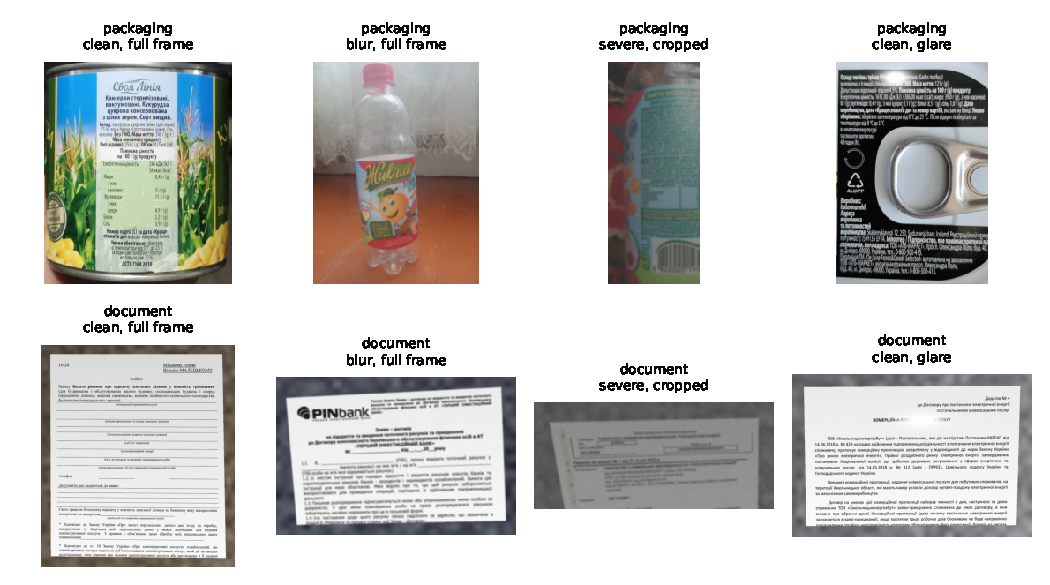
\includegraphics[width=\textwidth]{figures/fig_examples.pdf}
\caption{Example stimuli from the three genres under different quality and framing conditions. All text is Ukrainian, and the ground truth records every character and whether it is visible in the final frame.}\label{fig:examples}
\end{figure}

\subsection{Models and prompts}\label{sec:models}

We queried four production models from one vendor, spanning its capability and price range: Claude Haiku~5.5, Sonnet~5.5 and Opus~5.5 on all \NImages{} images, and Claude Fable~5.1, the most expensive model, on a balanced subset of \NFableImages{} images (replicates 0 and 1 of every design cell). All calls used the vendor's command-line client in non-interactive mode with default sampling settings, no tools and a short system prompt in Ukrainian: \foreignlanguage{ukrainian}{«Ти — сервіс опису зображень для незрячих і слабозорих користувачів. Відповідай українською мовою.»} (``You are an image-description service for blind and low-vision users. Answer in Ukrainian.''). Images were passed under opaque hashed file names so that the file name could not reveal the condition.

Two user prompts were used, each in a separate call without shared context. The \emph{description} prompt imitates a blind user's request: \foreignlanguage{ukrainian}{«Я незряча людина. Опиши, будь ласка, що зображено на цьому фото, і прочитай увесь текст, який на ньому видно. Увесь прочитаний текст наводь дослівно в лапках «…».»} (``I am a blind person. Please describe what is shown in this photo and read all the text that is visible on it. Give all the text you read verbatim in «…» quotation marks.''). The request for guillemets makes the claimed text machine-extractable without an additional model. The \emph{transcription} prompt asks for a verbatim line-by-line transcription, forbids corrections and completions, asks for a placeholder \foreignlanguage{ukrainian}{[нерозбірливо]} (``illegible'') where text is cut off, covered or unreadable, and asks for a ``(?)'' after any uncertain word. It serves both as a mitigation condition and as a run-time re-reading signal for detection.

\subsection{Extracting and labelling claimed text}\label{sec:labelling}

From each description we extract every guillemet-quoted span; an opening guillemet runs to the next closing one on the same line, so nested quotation marks cannot absorb descriptive prose. Straight and curly double quotes are also accepted. Bracketed or parenthesised remarks inside a quotation (e.g., \foreignlanguage{ukrainian}{«Осо[закрито пальцем] рахунок»}) are treated as annotations and removed, as are quotations that consist only of meta-words such as ``covered'' or of a single letter. Duplicate spans within a response are counted once. From each transcription, all lines are used after removing placeholders. Text is normalised by lower-casing, unifying apostrophe variants and mapping Latin look-alike letters inside Cyrillic words to Cyrillic. It is then split into letter and digit tokens. Digits separated by dots, colons or commas are merged, so dates, times and prices compare as units. Phone-like digit runs are also merged regardless of spacing, and leading zeros are dropped.

Each claimed token $o$ receives one label from the ground truth of its image:
\begin{itemize}
\item \textbf{correct}: $o$ equals a visible token or a readable partial token, or $o$ is an explicit fragment (at least two characters) of a visible token or a contiguous run of the visible characters of a partial token;
\item \textbf{completion}: $o$ equals the full form of a token at least one of whose characters is hidden, i.e., the text is true but the camera did not capture it;
\item \textbf{misreading}: none of the above, but $o$ is within a normalised edit similarity of 0.5 of some ground-truth token, i.e., printed text was rendered wrongly;
\item \textbf{fabrication}: no ground-truth token is that similar, i.e., the text was invented.
\end{itemize}
A \emph{hallucinated} token is a misreading or a fabrication; \emph{unsupported} tokens additionally include completions. Misreadings are sub-typed as \emph{digit} errors, \emph{Ukrainian-letter} substitutions (the claimed and printed words differ only in \foreignlanguage{ukrainian}{і/и, ї/і, є/е, ґ/г} or contain letters that exist only in Russian), \emph{lexicalisations} (the claimed form is a real word or a known name but the printed one is not), and other substitutions. We also record whether the sentence containing a quotation carries a hedging cue (e.g., \foreignlanguage{ukrainian}{«ймовірно»}, \foreignlanguage{ukrainian}{«схоже»}, \foreignlanguage{ukrainian}{«нечітко»}, ``probably'', ``looks like'', ``blurry''). Matching against the image's token set rather than a forced alignment is deliberately conservative: a wrong number that happens to occur elsewhere on the same panel counts as correct. The reported rates are therefore lower bounds.

\paragraph{Audit.} To estimate the labeller's precision, the first author inspected a stratified random sample of \NAudit{} labelled tokens from all four models, with the quoted span and the printed line side by side, and judged whether each label was right.

\subsection{Detectors}\label{sec:detectors}

For each token quoted in a description, five signals are computed without access to the ground truth:
\begin{enumerate}
\item \emph{re-reading}: the token is absent from the same model's transcription of the same image; the variant \emph{re-reading uncertainty} fires when the transcription marks the token with ``(?)'';
\item \emph{cross-model}: the fraction of the other two main models whose description or transcription of the image does not contain the token;
\item \emph{OCR}: one minus the best normalised edit similarity between the token and any token Tesseract~5.5 (\texttt{tessdata\_best} Ukrainian model, page-segmentation modes 3 and 11 pooled) reads in the image~\cite{smith2007overview};
\item \emph{lexicon}: the token is not in the Ukrainian frequency list;
\item \emph{hedging}: the quoting sentence carries a hedging cue.
\end{enumerate}
Each signal is evaluated alone by the area under the ROC curve (AUROC)~\cite{hanley1982meaning}, and all signals are combined, together with the token's length and digit status, in a class-balanced logistic regression. Its scores are obtained by five-fold cross-validation with folds grouped by image, so that no image contributes to both training and testing. We report AUROC, average precision and, for deployment, the share of hallucinated tokens caught at fixed false-flag rates of 5, 10 and 20\% on correct tokens. We also evaluate a simple rule that needs no training: flag a token if the model's re-reading lacks it, or if neither OCR nor a majority of the other models confirms it.

\subsection{Statistics}\label{sec:stats}

Proportions are reported with Wilson 95\% score intervals~\cite{wilson1927probable}. Because tokens are clustered within images, we additionally report percentile intervals from a cluster bootstrap over images~\cite{efron1979bootstrap} (1000 resamples for rates and 300 for AUROC). Paired comparisons of the description and transcription prompts on the same images use the exact McNemar test on image-level outcomes. All analysis code and the response-free aggregate results are released (see Declarations). Raw model responses are withheld from the repository but can be regenerated with the released scripts.


\backmatter

\bmhead{Acknowledgements}

We thank the developers of Tesseract, the \texttt{tessdata\_best} models and the FrequencyWords lists, and the designers of the open-licensed Cyrillic fonts used to render the stimuli.

\section*{Declarations}

\bmhead{Funding}
No funding was received for conducting this study.

\bmhead{Competing interests}
The authors have no competing interests to declare that are relevant to the content of this article.

\bmhead{Ethics approval and consent to participate}
Not applicable. The study used only synthetic images and automated model queries; no human participants or personal data were involved.

\bmhead{Consent for publication}
Not applicable.

\bmhead{Data availability}
The stimulus images, the complete ground truth (every character, its slot category and its visibility), and the response-free aggregate results are available in the project repository, \url{https://github.com/rzats/universal-access-in-2026}. Raw model responses are not redistributed. They can be regenerated with the released scripts, subject to the model provider's terms.

\bmhead{Materials availability}
Not applicable.

\bmhead{Code availability}
The stimulus generator, model-query, OCR, labelling, analysis and figure scripts are available in the same repository.

\bmhead{Author contribution}
R.Z.: conceptualisation, methodology, software, formal analysis, writing (original draft). R.Za.: conceptualisation, validation, accessibility domain expertise, writing (review and editing). Both authors read and approved the final manuscript.

\bmhead{Use of generative AI}
During the preparation of this work the authors used Claude (Anthropic) to proofread the manuscript and check grammar and spelling. The Claude models evaluated as the objects of study are described in Section~\ref{sec:models}.

\bibliography{refs}

\end{document}
